\documentclass[tikz,border=2mm]{standalone}
\usepackage[T1]{fontenc}
\usepackage[swedish,english]{babel}
\usepackage{tikz}
\usetikzlibrary{arrows,positioning}
\usepackage{pgfplots}
\usepackage{amsmath,mathtools}
\usepgfplotslibrary{fillbetween}
\begin{document}
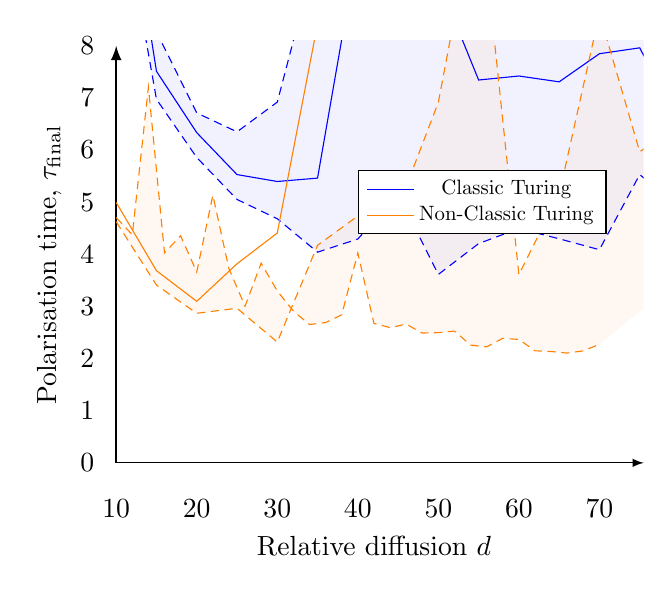
\begin{tikzpicture}
\begin{axis}[
    %hide axis,
    %axis lines* = left,
    %axis lines=left, xtick=\empty, ytick=\empty.
    axis line style={draw=none},
    tick style={draw=none},
    xticklabel style={yshift=-0.1mm},
    xmin = 8.5,
   xmax =75.5,
    ymin = -0.5,
    ymax = 8.1,
    %grid=both,
    %xtick = {1,0.95,...,0.6},
    ytick = {0,1,...,20},    
    %xticklabels = {{zero},$\alpha$,$\varphi$},
   %xlabel style={at={(axis cs:0.61,7)},anchor=east,align=center},
    %ylabel style={at={(axis cs:1.00,35)},anchor=north,rotate=0},
	xlabel = {Relative diffusion $d$},
        ylabel = {Polarisation time, $\tau_{\textrm{final}}$},
    legend style={at={(axis cs:40,5)},anchor=west,cells={align=center},nodes={scale=0.75}},
    %x dir=reverse
    %legend entries = {Decreasing the inactivation rate $k_{-2}$}
]
%-------------------------------------------------------------------------------------------------
% AXES
\draw[->,-latex, thick] (axis cs: 10,0) -- (axis cs: 10,8); % y-axis
\draw[->,-latex] (axis cs: 10,0) -- (axis cs: 75.5,0); % x-axis
%-------------------------------------------------------------------------------------------------
%-------------------------------------------------------------------------------------------------
% Classical 
%-------------------------------------------------------------------------------------------------
\addplot[forget plot,densely dashed,color=blue,name path=UppolTimeClassical] coordinates {
		(10.0000	,	13.8070	)
		(15.0000	,	8.2663	)
		(20.0000	,	6.7126	)
		(25.0000	,	6.3496	)
		(30.0000	,	6.9199	)
		(35.0000	,	9.8654	)
		(40.0000	,	12.5469	)
		(45.0000	,	13.2513	)
		(50.0000	,	12.4028	)
		(55.0000	,	10.9015	)
		(60.0000	,	11.2219	)
		(65.0000	,	11.6050	)
		(70.0000	,	18.2605	)
		(75.0000	,	16.3231	)
		(80.0000	,	8.6555	)
		(85.0000	,	16.0681	)
		(90.0000	,	12.0466	)
		(95.0000	,	12.3425	)
		(100.0000	,	15.8997	)
		(105.0000	,	16.1367	)
		(110.0000	,	13.0150	)
		(115.0000	,	13.9863	)
		(120.0000	,	13.5020	)
		(125.0000	,	13.8966	)
		(130.0000	,	11.6090	)
		(135.0000	,	11.8488	)
		(140.0000	,	15.0951	)
		(145.0000	,	22.0615	)
		(150.0000	,	28.7503	)
		(155.0000	,	25.8918	)
		(160.0000	,	33.1674	)
};

\addplot[color=blue] coordinates {
		(10.0000	,	12.4173	)
		(15.0000	,	7.5114	)
		(20.0000	,	6.3345	)
		(25.0000	,	5.5299	)
		(30.0000	,	5.3972	)
		(35.0000	,	5.4620	)
		(40.0000	,	9.8896	)
		(45.0000	,	9.1300	)
		(50.0000	,	9.2474	)
		(55.0000	,	7.3439	)
		(60.0000	,	7.4207	)
		(65.0000	,	7.3088	)
		(70.0000	,	7.8486	)
		(75.0000	,	7.9611	)
		(80.0000	,	6.4674	)
		(85.0000	,	9.3734	)
		(90.0000	,	7.8614	)
		(95.0000	,	8.6665	)
		(100.0000	,	10.2711	)
		(105.0000	,	10.1026	)
		(110.0000	,	9.9021	)
		(115.0000	,	11.2298	)
		(120.0000	,	10.9722	)
		(125.0000	,	10.8237	)
		(130.0000	,	8.8464	)
		(135.0000	,	9.5047	)
		(140.0000	,	10.1898	)
		(145.0000	,	9.9682	)
		(150.0000	,	10.0662	)
		(155.0000	,	9.5947	)
		(160.0000	,	10.9956	)
};

\addplot[forget plot,densely dashed,color=blue,name path=DownpolTimeClassical] coordinates {
		(10.0000	,	11.3512	)
		(15.0000	,	6.9742	)
		(20.0000	,	5.8575	)
		(25.0000	,	5.0527	)
		(30.0000	,	4.6825	)
		(35.0000	,	4.0414	)
		(40.0000	,	4.2929	)
		(45.0000	,	5.1524	)
		(50.0000	,	3.6142	)
		(55.0000	,	4.2065	)
		(60.0000	,	4.4947	)
		(65.0000	,	4.2979	)
		(70.0000	,	4.0887	)
		(75.0000	,	5.5302	)
		(80.0000	,	4.8708	)
		(85.0000	,	5.0326	)
		(90.0000	,	5.4865	)
		(95.0000	,	4.4223	)
		(100.0000	,	7.0748	)
		(105.0000	,	5.5108	)
		(110.0000	,	5.6310	)
		(115.0000	,	7.4391	)
		(120.0000	,	7.9455	)
		(125.0000	,	6.7780	)
		(130.0000	,	5.0482	)
		(135.0000	,	5.6751	)
		(140.0000	,	6.6782	)
		(145.0000	,	5.2923	)
		(150.0000	,	6.7368	)
		(155.0000	,	6.3886	)
		(160.0000	,	7.1456	)
};
\addplot[blue!50,opacity=0.1,forget plot] fill between[of=UppolTimeClassical and DownpolTimeClassical];

\addlegendentry{Classic Turing}% Add to legend
%-------------------------------------------------------------------------------------------------
% Non-classical
%-------------------------------------------------------------------------------------------------
\addplot[forget plot,densely dashed,color=orange,name path=UppolTimeNonClassical] coordinates {
		(10.0000	,	4.7040	)
		(12.0000	,	4.3770	)
		(14.0000	,	7.2075	)
		(16.0000	,	4.0269	)
		(18.0000	,	4.3563	)
		(20.0000	,	3.6606	)
		(22.0000	,	5.1343	)
		(24.0000	,	3.7229	)
		(26.0000	,	3.0060	)
		(28.0000	,	3.8307	)
		(30.0000	,	3.2972	)
		(32.0000	,	2.9111	)
		(34.0000	,	2.6529	)
		(36.0000	,	2.6911	)
		(38.0000	,	2.8380	)
		(40.0000	,	4.0261	)
		(42.0000	,	2.6736	)
		(44.0000	,	2.5947	)
		(46.0000	,	2.6606	)
		(48.0000	,	2.4907	)
		(50.0000	,	2.4974	)
		(52.0000	,	2.5273	)
		(54.0000	,	2.2595	)
		(56.0000	,	2.2249	)
		(58.0000	,	2.3890	)
		(60.0000	,	2.3674	)
		(62.0000	,	2.1494	)
		(64.0000	,	2.1356	)
		(66.0000	,	2.1058	)
		(68.0000	,	2.1484	)
		(70.0000	,	2.2739	)
};

\addplot[color=orange] coordinates {
		(10.0000	,	4.9950	)
		(15.0000	,	3.6863	)
		(20.0000	,	3.0982	)
		(25.0000	,	3.8183	)
		(30.0000	,	4.4089	)
		(35.0000	,	8.4180	)
		(40.0000	,	9.6850	)
		(45.0000	,	11.0226	)
		(50.0000	,	13.2655	)
		(55.0000	,	12.2860	)
		(60.0000	,	10.6073	)
		(65.0000	,	10.1577	)
		(70.0000	,	12.9037	)
		(75.0000	,	10.9900	)
		(80.0000	,	11.0068	)
		(85.0000	,	11.3503	)
		(90.0000	,	15.1204	)
		(95.0000	,	14.1499	)
		(100.0000	,	16.5177	)
		(105.0000	,	16.5502	)
		(110.0000	,	16.3277	)
		(115.0000	,	16.4061	)
		(120.0000	,	16.7902	)
		(125.0000	,	15.7433	)
		(130.0000	,	17.9356	)
		(135.0000	,	17.6099	)
		(140.0000	,	20.6761	)
		(145.0000	,	19.3805	)
		(150.0000	,	18.0079	)
		(155.0000	,	26.5605	)
		(160.0000	,	25.5344	)
};

\addplot[forget plot,densely dashed,color=orange,name path=DownpolTimeNonClassical] coordinates {
		(10.0000	,	4.6257	)
		(15.0000	,	3.4104	)
		(20.0000	,	2.8692	)
		(25.0000	,	2.9653	)
		(30.0000	,	2.3168	)
		(35.0000	,	4.1735	)
		(40.0000	,	4.7351	)
		(45.0000	,	4.8943	)
		(50.0000	,	6.9172	)
		(55.0000	,	10.9986	)
		(60.0000	,	3.6125	)
		(65.0000	,	5.1512	)
		(70.0000	,	8.6213	)
		(75.0000	,	5.9681	)
		(80.0000	,	6.4743	)
		(85.0000	,	7.0185	)
		(90.0000	,	7.7166	)
		(95.0000	,	9.4738	)
		(100.0000	,	10.7370	)
		(105.0000	,	8.6114	)
		(110.0000	,	10.2740	)
		(115.0000	,	13.2730	)
		(120.0000	,	10.6487	)
		(125.0000	,	10.4863	)
		(130.0000	,	11.3547	)
		(135.0000	,	12.9647	)
		(140.0000	,	10.2379	)
		(145.0000	,	11.9698	)
		(150.0000	,	10.2452	)
		(155.0000	,	10.0773	)
		(160.0000	,	13.6793	)
};
\addplot[orange!50,opacity=0.1,forget plot] fill between[of=UppolTimeNonClassical and DownpolTimeNonClassical];

\addlegendentry{Non-Classic Turing}% Add to legend
\end{axis}

\end{tikzpicture}



\end{document}
